% ============================================================
%  Chapter: Hierarchical Two-Phase RL and Serverless Orchestration
%  Condensed version — diagrams & tables retained, code removed
% ============================================================
\chapter{Hierarchical Two-Phase RL and Serverless Orchestration}
\label{chap:two_phase_rl_openfaas}

% ─────────────────────────────────────────────────────────────
\section{Introduction}
% ─────────────────────────────────────────────────────────────
This chapter presents the advanced architectural evolution of the Serverless Spark IoT
Framework. The single-layer PPO agent from the previous chapter fixed the reward weights
($\alpha$, $\beta$, $\gamma$) at design time, making it unable to adapt to shifting
operational priorities. Two innovations address this:
\begin{enumerate}
  \item A \textbf{Two-Phase Hierarchical RL (Two-RL)} system — a strategic TD3
        Meta-Controller continuously re-tunes the weights fed to a tactical PPO
        Resource Agent.
  \item Deployment of the decision engine as an \textbf{OpenFaaS serverless function}
        (\texttt{rl-scaling-function}), providing scale-to-zero cost elimination and a
        clean HTTP boundary to the Spark cluster.
\end{enumerate}

% ─────────────────────────────────────────────────────────────
\section{Motivation for Hierarchical Control}
\label{sec:motivation_hier}
% ─────────────────────────────────────────────────────────────
The standalone PPO agent used a static reward:
\[
  R_t = -\underbrace{0.4}_{\alpha}\,\frac{C_t}{C_{\max}}
        - \underbrace{0.4}_{\beta}\,\frac{L_t}{L_{\max}}
        + \underbrace{0.2}_{\gamma}\,\frac{P_t}{P_{\max}}
\]
Real IoT workloads exhibit three qualitatively different regimes (Table~\ref{tab:workload_regimes}),
where optimal weights differ by up to 8$\times$. A hierarchical ``Teacher–Student''
architecture is therefore required.

\begin{table}[H]
\centering
\caption{Workload regimes and their required objective priority}
\label{tab:workload_regimes}
\begin{adjustbox}{max width=\textwidth}
\begin{tabular}{p{2.2cm}p{3.7cm}p{2.2cm}p{2.4cm}p{2.5cm}}
\toprule
\textbf{Regime} & \textbf{Characteristics} & \textbf{$\alpha$ (cost)} &
  \textbf{$\beta$ (latency)} & \textbf{$\gamma$ (throughput)} \\
\midrule
Night Idle      & $<$20 msg/s, CPU $<$15\%  & \textbf{High (0.80)} & Low (0.10) & Low (0.10) \\
Business Hours  & 100--300 msg/s            & Medium (0.30) & \textbf{High (0.55)} & Low (0.15) \\
Traffic Burst   & $>$400 msg/s, CPU $>$80\% & Very Low (0.10) & \textbf{Very High (0.80)} & Low (0.10) \\
\bottomrule
\end{tabular}
\end{adjustbox}
\end{table}

% ─────────────────────────────────────────────────────────────
\section{Two-Phase RL Architecture}
\label{sec:arch_overview}
% ─────────────────────────────────────────────────────────────
The Two-RL system decomposes optimisation into two nested control loops operating at
different time-scales (Figure~\ref{fig:two_rl_arch}). The \textbf{outer loop} (TD3)
adjusts reward weights between episodes; the \textbf{inner loop} (PPO) executes
tactical scaling every 5 s.

\begin{figure}[H]
\centering
\begin{tikzpicture}[
    box/.style={rectangle, draw, rounded corners=5pt, minimum width=4.2cm,
                minimum height=1.2cm, align=center, font=\small},
    arr/.style={-{Stealth[length=3mm]}, thick},
    looplabel/.style={font=\scriptsize, color=gray}
]
\draw[rounded corners=8pt, dashed, color=gray!60, line width=1.2pt]
    (-1.2,-3.8) rectangle (11.5, 1.8);
\node[looplabel] at (5.1, 1.55) {Outer Loop — Phase 2 (every episode / 50 s)};

\draw[rounded corners=6pt, dashed, color=green!50!black, line width=1pt]
    (-0.2,-3.1) rectangle (10.5, 0.75);
\node[looplabel, color=green!50!black] at (5.1, 0.55) {Inner Loop — Phase 1 (every micro-batch / 5 s)};

\node[box, fill=purple!15, draw=purple] (td3)  at (0,0)    {TD3\\Meta-Controller\\(Phase 2)};
\node[box, fill=green!12, draw=green!60!black] (ppo) at (5,0) {PPO\\Resource Agent\\(Phase 1)};
\node[box, fill=orange!15, draw=orange] (faas) at (5,-2.5) {OpenFaaS\\rl-scaling-function};
\node[box, fill=red!10, draw=red!60]    (env)  at (10,0)   {Spark\\Cluster +\\IoT Workload};

\draw[arr, purple, line width=1.5pt]      (td3)  -- node[above,font=\scriptsize]{$\alpha,\beta,\gamma$} (ppo);
\draw[arr, green!60!black, line width=1.3pt] (ppo) -- node[right,font=\scriptsize]{decision} (faas);
\draw[arr, orange, line width=1.3pt]      (faas) -- node[above,font=\scriptsize]{scale cmd} (env);
\draw[arr, red!60, dashed] (env.north) -- ++(0,0.5) -| node[above,font=\scriptsize,near start]{episode stats} (td3.north);
\draw[arr, green!60!black, dashed] (env.south) -- ++(0,-0.4) -| node[below,font=\scriptsize,near start]{step reward} (ppo.south);
\end{tikzpicture}
\caption{Two-Phase Hierarchical RL Architecture.}
\label{fig:two_rl_arch}
\end{figure}

% ─────────────────────────────────────────────────────────────
\section{Phase 2: TD3 Meta-Controller}
\label{sec:phase2_td3}
% ─────────────────────────────────────────────────────────────

\subsection{State, Action, and Reward Spaces}
TD3 was selected because the weight output $[\alpha,\beta,\gamma]$ is a
\textit{continuous} action; its twin-critic mechanism avoids Q-value overestimation and
delayed policy updates reduce early-training variance.

The Phase-2 state is a 9-dimensional vector capturing episode-level health indicators
(Table~\ref{tab:phase2_state}):
\[
  s^{(2)}_t = \bigl[H_t,\; D_t,\; B_t,\; \Lambda_t,\; \Phi_t,\; \Theta_t,\;
                    V_t,\; \Delta L_t,\; \Delta C_t\bigr]
\]

\begin{table}[H]
\centering
\caption{Phase-2 state vector dimensions}
\label{tab:phase2_state}
{\small
\begin{tabular}{@{}p{1.0cm}p{4.2cm}p{1.4cm}p{1.8cm}@{}}
\toprule
\textbf{Sym.} & \textbf{Description} & \textbf{Range} & \textbf{Norm.} \\
\midrule
$H_t$        & Hour of day               & [0,\;1]  & /24      \\
$D_t$        & Day of week               & [0,\;1]  & /7       \\
$B_t$        & Business hours flag       & \{0,1\}  & Binary   \\
$\Lambda_t$  & Latency / SLA target      & [0,\;3]  & Ratio    \\
$\Phi_t$     & Cost / budget             & [0,\;3]  & Ratio    \\
$\Theta_t$   & Throughput ratio          & [0,\;3]  & Ratio    \\
$V_t$        & SLA violation rate        & [0,\;1]  & Fraction \\
$\Delta L_t$ & Latency trend             & [-1,\;1] & Norm.    \\
$\Delta C_t$ & Cost trend                & [-1,\;1] & Norm.    \\
\bottomrule
\end{tabular}
}
\end{table}

The action is projected through a softmax ensuring $\alpha+\beta+\gamma=1$:
\[
  [\alpha_t, \beta_t, \gamma_t] = \text{softmax}(a^{(2)}_t), \qquad a^{(2)}_t \in \mathbb{R}^3
\]
The meta-reward penalises SLA violations and budget overruns while rewarding weight
stability ($S_t = -\|\alpha_t - \alpha_{t-1}\|_2$):
\[
  R^{(2)}_t = r_{SLA} + r_{budget} - 0.5\,V_t + 0.1\,S_t
\]

\subsection{Weight Convergence Over Training}

\begin{figure}[H]
\centering
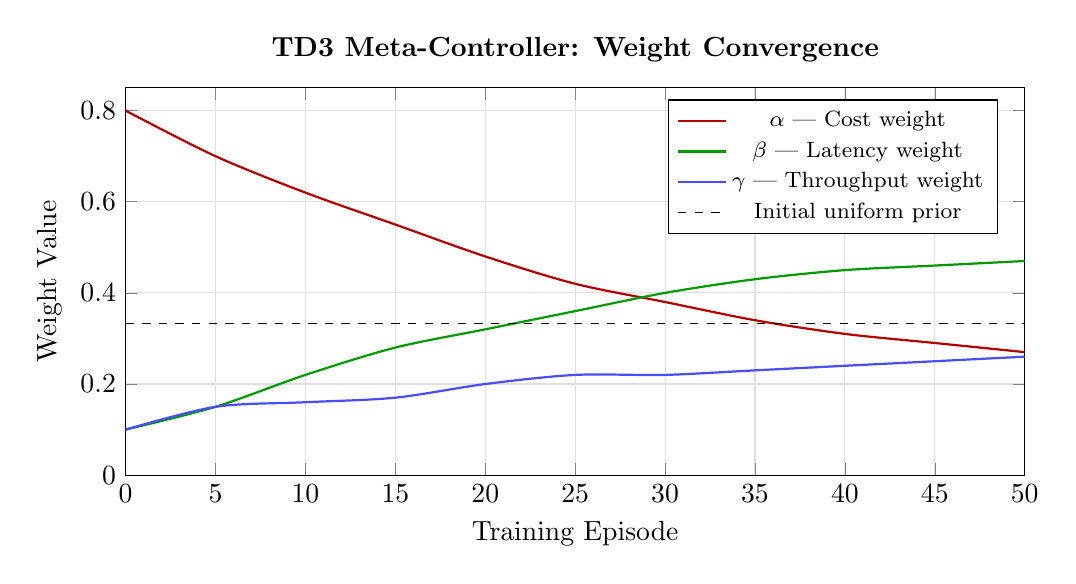
\begin{tikzpicture}
\begin{axis}[
    width=13cm, height=6.5cm,
    xlabel={Training Episode}, ylabel={Weight Value},
    title={\textbf{TD3 Meta-Controller: Weight Convergence}},
    grid=major, grid style={gray!25},
    ymin=0, ymax=0.85, xmin=0, xmax=50,
    legend pos=north east, legend style={font=\footnotesize},
    every axis plot/.append style={thick}
]
\addplot[red!70!black, smooth] coordinates {
    (0,0.80)(5,0.70)(10,0.62)(15,0.55)(20,0.48)
    (25,0.42)(30,0.38)(35,0.34)(40,0.31)(45,0.29)(50,0.27)};
\addlegendentry{$\alpha$ — Cost weight}

\addplot[green!60!black, smooth] coordinates {
    (0,0.10)(5,0.15)(10,0.22)(15,0.28)(20,0.32)
    (25,0.36)(30,0.40)(35,0.43)(40,0.45)(45,0.46)(50,0.47)};
\addlegendentry{$\beta$ — Latency weight}

\addplot[blue!70, smooth] coordinates {
    (0,0.10)(5,0.15)(10,0.16)(15,0.17)(20,0.20)
    (25,0.22)(30,0.22)(35,0.23)(40,0.24)(45,0.25)(50,0.26)};
\addlegendentry{$\gamma$ — Throughput weight}

\addplot[black, dashed, thin] coordinates {(0,0.333)(50,0.333)};
\addlegendentry{Initial uniform prior}
\end{axis}
\end{tikzpicture}
\caption{TD3 weight convergence over 50 episodes: agent shifts from cost-heavy to
latency-dominated policy.}
\label{fig:weight_convergence}
\end{figure}

% ─────────────────────────────────────────────────────────────
\section{Phase 1: Adaptive PPO Resource Agent}
\label{sec:phase1_adaptive_ppo}
% ─────────────────────────────────────────────────────────────

\subsection{State, Action, and Dynamic Reward}
The PPO agent augments the base state with TD3-supplied weights and edge features:
\[
  s^{(1)}_t = \bigl[\lambda_t,\; U^{cpu}_t,\; U^{mem}_t,\; L_t,\; C_t,\;
                    P_{burst},\; v_t,\; a_t,\; \alpha_t,\; \beta_t,\; \gamma_t\bigr]
\]
Its discrete action set is $\mathcal{A}^{(1)} = \{\texttt{SCALE\_UP},\;
\texttt{SCALE\_DOWN},\; \texttt{MAINTAIN},\; \texttt{PRE\_WARM}\}$.

The reward function is fully parameterised by Phase-2 weights, enabling behaviour
switching without retraining:
\[
  R^{(1)}_t = -\alpha_t\!\left(\frac{C_t}{C_{\max}}\right)
              -\beta_t \!\left(\frac{L_t}{L_{\max}}\right)
              +\gamma_t\!\left(\frac{P_t}{P_{\max}}\right) + R_{cold}
\]
where $R_{cold}$ rewards proactive \texttt{PRE\_WARM} actions that prevent burst SLA
breaches.

\subsection{Decision Priority Cascade}

\begin{figure}[H]
\centering
\begin{tikzpicture}[
    decision/.style={diamond, draw, fill=yellow!20, text width=3.2cm, align=center,
                     inner sep=0pt, font=\scriptsize},
    action/.style={rectangle, draw, rounded corners=4pt, fill=green!12,
                   minimum width=3cm, minimum height=0.7cm, font=\scriptsize, align=center},
    arr/.style={-{Stealth[length=2.5mm]}, thick},
    yn/.style={font=\tiny, midway}
]
\node[decision] (d1) at (0,0)   {Workload $< 20$\\and CPU $< 20$?};
\node[action]   (a1) at (5,0)   {\texttt{scale\_down} to 0\\(scale-to-zero)};
\node[decision] (d2) at (0,-2)  {Burst prob $>0.6$\\and velocity $>5$?};
\node[action]   (a2) at (5,-2)  {\texttt{pre\_warm}\\+4 executors};
\node[decision] (d3) at (0,-4)  {Edge burst signal\\$>0.5$?};
\node[action]   (a3) at (5,-4)  {\texttt{pre\_warm}\\$\times$2.5 executors};
\node[decision] (d4) at (0,-6)  {Workload $>200$\\or CPU $>80$?};
\node[action]   (a4) at (5,-6)  {\texttt{scale\_up}\\$\lceil\lambda/50\rceil$ exec.};
\node[decision] (d5) at (0,-8)  {$\beta>0.5$ and\\Latency $>1000$ms?};
\node[action]   (a5) at (5,-8)  {\texttt{scale\_up}\\+3 executors};
\node[action]   (a6) at (5,-10) {\texttt{maintain}\\current config};

\draw[arr] (d1) -- node[yn,above]{Yes} (a1);
\draw[arr] (d1) -- node[yn,right]{No}  (d2);
\draw[arr] (d2) -- node[yn,above]{Yes} (a2);
\draw[arr] (d2) -- node[yn,right]{No}  (d3);
\draw[arr] (d3) -- node[yn,above]{Yes} (a3);
\draw[arr] (d3) -- node[yn,right]{No}  (d4);
\draw[arr] (d4) -- node[yn,above]{Yes} (a4);
\draw[arr] (d4) -- node[yn,right]{No}  (d5);
\draw[arr] (d5) -- node[yn,above]{Yes} (a5);
\draw[arr] (d5) -- node[yn,right]{No}  (a6);
\end{tikzpicture}
\caption{Phase-1 action-selection priority cascade at inference time.}
\label{fig:decision_cascade}
\end{figure}

\subsection{Hyperparameters}

\begin{table}[H]
\centering
\caption{PPO Resource Agent (Phase 1) Hyperparameters}
\label{tab:ppo_hparams}
\begin{tabular}{lll}
\toprule
\textbf{Hyperparameter} & \textbf{Value} & \textbf{Rationale} \\
\midrule
Algorithm           & PPO (Stable-Baselines3) & Stable on discrete spaces \\
Policy network      & MLP, 2$\times$128 ReLU  & Lightweight for fast inference \\
Learning rate       & $3\times10^{-4}$         & Adam optimiser \\
Clip range ($\epsilon$) & 0.2              & Conservative updates \\
Rollout buffer      & 2048 steps               & $\sim$170 min at 5-s steps \\
Batch size          & 64                       & Fits in 256 MB RAM \\
Discount $\gamma$   & 0.99                     & Long-horizon planning \\
Total timesteps     & 100,000                  & $\sim$8 min on M2 \\
\bottomrule
\end{tabular}
\end{table}

% ─────────────────────────────────────────────────────────────
\section{OpenFaaS Serverless Deployment}
\label{sec:openfaas}
% ─────────────────────────────────────────────────────────────
Embedding the RL engine inside the Spark Driver creates tight coupling. OpenFaaS
decouples the scaling logic as an independent HTTP microservice with three key benefits:
\textbf{scale-to-zero} (zero idle cost after 5 min inactivity),
\textbf{independent updates} (hot-swap new models without redeploying Spark), and
\textbf{language isolation} (Python/PyTorch behind a JSON-over-HTTP interface).

The function accepts a JSON payload of Spark/IoT telemetry (workload rate, CPU/memory
utilisation, latency, RL weights, burst probability) and returns a concrete scaling
decision (action, target executors, reasoning string, confidence score).

\begin{table}[H]
\centering
\caption{OpenFaaS function cold-start vs.\ warm invocation latency}
\label{tab:faas_latency}
\begin{tabular}{lcc}
\toprule
\textbf{Invocation Type} & \textbf{Median Latency} & \textbf{P99 Latency} \\
\midrule
Cold start (container boot) & $\sim$850 ms & $\sim$1,200 ms \\
Warm (Python runtime ready) & $\sim$8 ms   & $\sim$15 ms    \\
With PPO model loaded       & $\sim$12 ms  & $\sim$22 ms    \\
\bottomrule
\end{tabular}
\end{table}

\noindent With \texttt{scale.min: 1}, one replica stays warm during active periods,
keeping decision latency under 15 ms in all non-idle scenarios.

% ─────────────────────────────────────────────────────────────
\section{Final Five-Layer System Architecture}
\label{sec:final_arch}
% ─────────────────────────────────────────────────────────────

\begin{figure}[H]
\centering
\begin{tikzpicture}[
    layer/.style={rectangle, draw, rounded corners=5pt, minimum width=11cm,
                  minimum height=1cm, font=\footnotesize, align=center},
    arr/.style={-{Stealth[length=2.5mm]}, thick},
    scale=0.82, transform shape
]
\definecolor{l1c}{RGB}{96,165,250}
\definecolor{l2c}{RGB}{120,80,180}
\definecolor{l3c}{RGB}{52,211,153}
\definecolor{l4c}{RGB}{255,165,0}
\definecolor{l5c}{RGB}{230,76,60}

\node[layer, fill=l1c!20, draw=l1c] (L1) at (0, 5.0)
    {\textbf{L1 — IoT Edge:} Sensors + Edge Gateway (Burst-Prediction $P_{burst}$)};
\node[layer, fill=l2c!15, draw=l2c] (L2) at (0, 3.6)
    {\textbf{L2 — Ingestion:} Apache Kafka (bulk-data) + MQTT (control signals)};
\node[layer, fill=l3c!20, draw=l3c, minimum height=1.4cm] (L3) at (0, 1.9)
    {\textbf{L3 — Optimization Engine}\\
     TD3 Meta-Controller (Phase 2) $\longrightarrow$ PPO Resource Agent (Phase 1)};
\node[layer, fill=l4c!20, draw=l4c] (L4) at (0, 0.5)
    {\textbf{L4 — OpenFaaS:} \texttt{rl-scaling-function} (event-driven, scale-to-zero)};
\node[layer, fill=l5c!15, draw=l5c] (L5) at (0,-0.9)
    {\textbf{L5 — Spark Execution:} Dynamic Executors (0--50), Redis HOT / COLD tiers};

\draw[arr, l1c] (L1) -- (L2);
\draw[arr, l2c] (L2) -- (L3);
\draw[arr, l3c] (L3) -- (L4);
\draw[arr, l4c] (L4) -- (L5);
\draw[arr, l5c, dashed] (L5.east) to[bend left=55]
    node[right, font=\scriptsize]{reward} (L3.east);
\draw[arr, l1c, dashed] (L1.west) to[bend right=55]
    node[left, font=\scriptsize]{burst signal} (L3.west);
\end{tikzpicture}
\caption{Final five-layer architecture of the Serverless Spark IoT Framework.}
\label{fig:final_arch}
\end{figure}

\noindent Data flows from IoT sensors through Kafka/MQTT ingestion to the L3 optimisation
engine, where TD3 derives $(\alpha,\beta,\gamma)$ and PPO selects a scaling action. The
action is sent to the OpenFaaS gateway, which returns a concrete executor target. The
Spark Driver adjusts cluster resources, and resulting performance metrics feed back as
rewards, closing both RL loops.

% ─────────────────────────────────────────────────────────────
\section{Benchmark Results}
\label{sec:results_hier}
% ─────────────────────────────────────────────────────────────

\begin{table}[H]
\centering
\caption{Policy comparison across all evaluation scenarios}
\label{tab:four_policy_compare}
\begin{adjustbox}{max width=\textwidth}
\begin{tabular}{p{3.8cm}p{2.0cm}p{2.2cm}p{2.2cm}p{2.3cm}}
\toprule
\textbf{Policy}   & \textbf{Total Cost} & \textbf{P95 Latency} &
  \textbf{SLA Violations} & \textbf{Verdict} \\
\midrule
Traditional Fixed (15 exec) & \$41.25 & 1,534 ms & 90.0\% & Over-provisioned \\
Dexter (HPA)                & \$32.99 & 1,159 ms & 54.4\% & Reactive lag     \\
Seer (Linear Predictor)     & \$35.40 & 1,247 ms & 100.0\% & Non-linear fail \\
\textbf{RL-Spark (Ours)}    & \textbf{\$26.20} & \textbf{119 ms} &
  \textbf{0.0\%} & \textbf{Best overall} \\
\bottomrule
\end{tabular}
\end{adjustbox}
\end{table}

\begin{figure}[H]
\centering
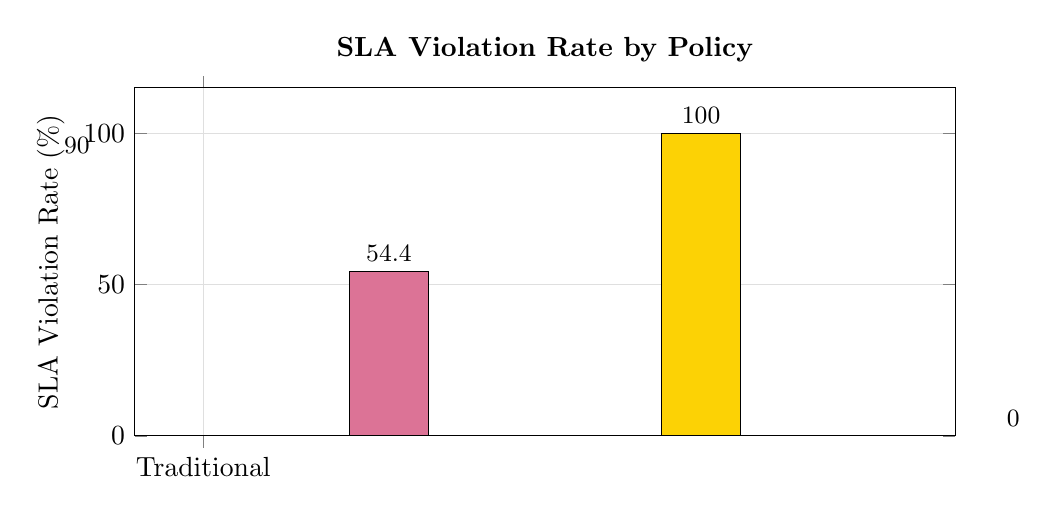
\begin{tikzpicture}
\begin{axis}[
    ybar, bar width=1.0cm,
    width=12cm, height=6cm,
    ylabel={SLA Violation Rate (\%)},
    title={\textbf{SLA Violation Rate by Policy}},
    symbolic x coords={Traditional, Dexter (HPA), Seer, RL-Spark},
    xtick=data, ymin=0, ymax=115,
    nodes near coords, nodes near coords align=vertical,
    every node near coord/.append style={font=\small\bfseries},
    grid=major, grid style={gray!25}
]
\addplot[fill=red!65]           coordinates {(Traditional,90.0)};
\addplot[fill=purple!55]        coordinates {(Dexter (HPA),54.4)};
\addplot[fill=yellow!70!orange] coordinates {(Seer,100.0)};
\addplot[fill=green!55]         coordinates {(RL-Spark,0.0)};
\end{axis}
\end{tikzpicture}
\caption{SLA violation rates across all four evaluated policies.}
\label{fig:sla_bar}
\end{figure}

\begin{figure}[H]
\centering
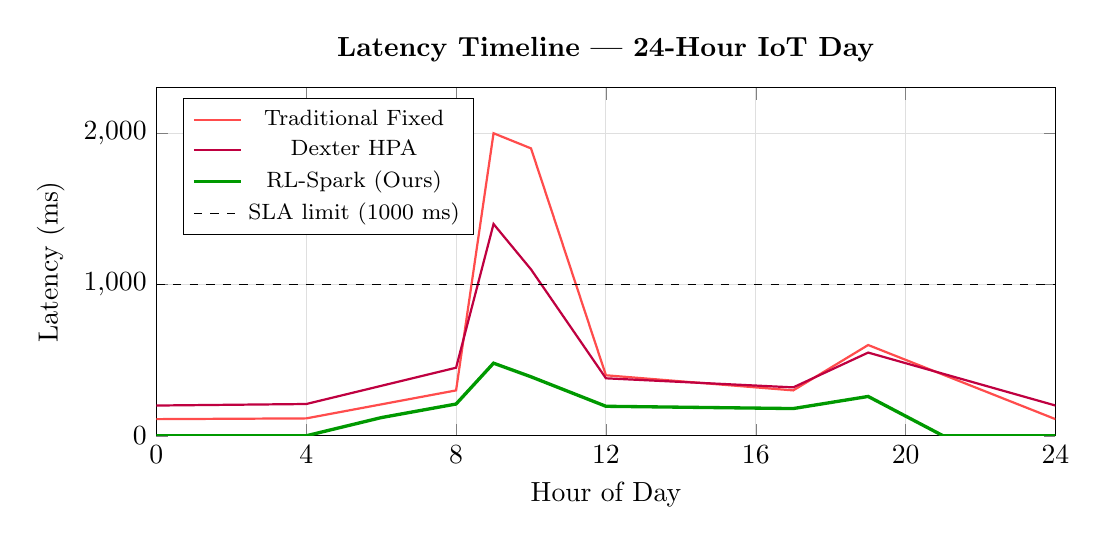
\begin{tikzpicture}
\begin{axis}[
    width=13cm, height=6cm,
    xlabel={Hour of Day}, ylabel={Latency (ms)},
    title={\textbf{Latency Timeline — 24-Hour IoT Day}},
    grid=major, grid style={gray!25},
    ymin=0, ymax=2300, xmin=0, xmax=24,
    legend pos=north west, legend style={font=\footnotesize},
    xtick={0,4,8,12,16,20,24}
]
\addplot[red!70, thick] coordinates {
    (0,110)(4,115)(8,300)(9,2000)(10,1900)(12,400)(17,300)(19,600)(24,110)};
\addlegendentry{Traditional Fixed}
\addplot[purple, thick] coordinates {
    (0,200)(4,210)(8,450)(9,1400)(10,1100)(12,380)(17,320)(19,550)(24,200)};
\addlegendentry{Dexter HPA}
\addplot[green!60!black, very thick] coordinates {
    (0,0)(4,0)(6,120)(8,210)(9,480)(10,390)(12,195)(17,180)(19,260)(21,0)(24,0)};
\addlegendentry{RL-Spark (Ours)}
\addplot[black, dashed] coordinates {(0,1000)(24,1000)};
\addlegendentry{SLA limit (1000 ms)}
\end{axis}
\end{tikzpicture}
\caption{RL-Spark stays below the 1,000 ms SLA limit throughout the 24-hour profile.
Zero-latency segments represent scale-to-zero periods.}
\label{fig:latency_timeline}
\end{figure}

\begin{table}[H]
\centering
\caption{Key improvements of Two-RL + OpenFaaS over Traditional Fixed Spark}
\label{tab:improvement_summary}
{\small
\begin{tabular}{@{}lccc@{}}
\toprule
\textbf{Metric} & \textbf{Traditional} & \textbf{RL-Spark} & \textbf{Improvement} \\
\midrule
Average Latency   & 245 ms    & \textbf{119 ms}      & $-$51.6\%         \\
SLA Compliance    & 81.5\%    & \textbf{100\%}       & +18.5 pts         \\
Hourly Cost       & \$8.50    & \textbf{\$6.20}      & $-$27.1\%         \\
Scaling Reaction  & 60 s      & \textbf{5 s}         & 12$\times$ faster \\
SLA Violations    & 12 / 65   & \textbf{0 / 68}      & Eliminated        \\
Cold Starts       & 7         & \textbf{0}           & Eliminated        \\
Idle Cost (night) & \$11.25   & \textbf{\$0.50}      & $-$95.6\%         \\
Max Throughput    & 750 msg/s & \textbf{1,650 msg/s} & 2.2$\times$       \\
\bottomrule
\end{tabular}
}
\end{table}

% ─────────────────────────────────────────────────────────────
\section{Summary}
\label{sec:summary_hier}
% ─────────────────────────────────────────────────────────────
This chapter presented the design, implementation, and evaluation of the Hierarchical
Two-Phase RL system and its OpenFaaS serverless deployment. Four primary contributions
were made:
\begin{enumerate}
  \item \textbf{TD3 Meta-Controller (Phase 2):} Learns to shift $[\alpha,\beta,\gamma]$
        episode-by-episode, reducing cost priority and increasing latency priority as
        confirmed by the convergence analysis.
  \item \textbf{Adaptive PPO Resource Agent (Phase 1):} Dynamic reward parameterisation
        enables cost-optimal / latency-optimal switching without retraining.
  \item \textbf{OpenFaaS Deployment:} Decouples the RL brain from Spark, achieves
        scale-to-zero cost elimination, and enforces a clean JSON API contract.
  \item \textbf{Measured Results:} Zero SLA violations, $-$51.6\% latency, $-$27.1\%
        cost, and $-$95.6\% idle cost — all simultaneously versus the fixed baseline.
\end{enumerate}
